\chapter{Staattisen tyyppitarkastuksen hyödyt}

\section{Virheiden havaitseminen}

Kenties tärkein tyyppijärjestelmän tehtävä on havaita ja estää
ohjelmoijan virheitä. Tyyppisäännöt eivät kykene tunnistamaan yleisesti
kaikenlaisia ongelmia koodissa — bugin lähteenä voi esimerkiksi olla
väärinymmärrys, jossa ohjelman vaatimukset on tulkittu ja toteutettu väärin.
Vaikka tyyppijärjestelmät eivät kykenisikään ehkäisemään kaikkia
virheitä, niillä voidaan kuitenkin havaita tietyn luokan virheet
systemaattisesti. Johdannossa annettiin esimerkki ohjelman virheellisestä
tilasta, jossa henkilön ikää kuvaavaan muuttujaan oli päätynyt tekstimuotoinen
arvo, \dblquoted{Matti}. Tämä on yksinkertainen esimerkki virheestä joka
olisi luultavasti helposti havaittavissa tyyppijärjestelmän
avulla. Myös dynaamiset tyyppijärjestelmät estävät tällaiset tyyppivirheet
suoritusaikana, mutta vasta jos virheen sisältävä osa koodia suoritetaan.
Tässä tutkielmassa esitellyt työkalut, mahdollisesti Closure–kääntäjää
lukuunottamatta, onkin kehitetty erityisesti estämään tyyppivirheitä
osana kehitysprosessia, jo ennen koodin suorittamista.

Kaikki kolme työkalua antaisivat käännösvirheen, jos esimerkeissä
\ref{lst:ostoskorin_hinta_closure} ja \ref{lst:ostoskorin_hinta_flow}
esiteltyä ostoskorifunktiota kutsuttaisiin virheellisesti esimerkiksi listalla
hintaa kuvaavia numeroita, sillä funktion parametrin on annotoitu olevan
lista \inlinecode{Ostos}-tyyppimääritelmän mukaisia objekteja. Koska
JavaScript on paitsi dynaamisesti myös heikosti tyypitetty,\newline
\colorbox{lightgray}{\lstinline|ostoskorinHinta([5, 10, 15])|} ei itse
asiassa aiheuttaisi suoritettaessa ohjelman\newline
keskeyttävää virhettä. Ilmaisu 
\colorbox{lightgray}{\lstinline|ostos.hinta|} on sallittu vaikka
muuttuja \colorbox{lightgray}{\lstinline|ostos|} olisikin arvoltaan numero
eikä \inlinecode{Ostos}-olio. Tällöin ilmaisun arvo olisi \colorbox{lightgray}{\lstinline|undefined|}
ja lausekkeen \colorbox{lightgray}{\lstinline|summa += ostos.hinta|} jälkeen
\colorbox{lightgray}{\lstinline|summa|}-muuttujan arvo olisi erityinen
ei-numeroa kuvaava \colorbox{lightgray}{\lstinline|NaN|} \cite{Ecma262NaN}.
Tyyppitarkistamisen merkitys korostuu erityisen hyödylliseksi
tämänkaltaisen ohjelmointivirheen kohdalla, sillä virhe ei välttämättä ole
muutoin helposti havaittavissa. Funktiokutsu ei aiheuttaisi helposti
todennettavaa suoritusaikaista virhettä, joten ei-toivottu palautusarvo
\colorbox{lightgray}{\lstinline|NaN|} saattaisi kiertää ohjelman
operaatioiden välillä pitkällekin aiheuttaen muita loogisia virheitä.

Vuonna 2017 tehdyssä tutkimuksessa \cite{ToTypeOrNotToType} TypeScriptin
ja Flown vaikutuksesta avoimen
lähdekoodin JavaScript-projekteihin havaittiin, että vähintään 15\%
ilmoitetuista ja korjatuista bugeista olisi voitu havaita ja välttää jos
projektin kehitykseen oltaisin käytetty jompaakumpaa näistä työkaluista.
Tutkimuksen arvioinnissa huomioitiin lisäksi, että tulos on tutkimusmenetelmästä
johtuen mitä luultavimmin alempi kuin tällaisen muutoksen tuoma todellinen
vaikutus. Tutkimus toteutettiin muuntamalla avoimen lähdekoodin
JavaScript-kirjastoja ensin staattisesti tyypitettyyn muotoon ja sitten
mittaamalla kuinka hyvin tyyppitarkastus havaitsi ennalta tunnettuja bugeja
aiheuttavan koodin. Sen ulkopuolelle jäivät bugit joita ei oltu vielä
korjattu tai havaittu, sekä bugit jotka kehittäjä oli havainnut jossain
kehitysvaiheessa ennen virheellisen ohjelman julkaisua. Staattisen
tyyppitarkastus luultavasti auttaisi vähentämään myös näitä bugeja.

\begin{figure}
\centering
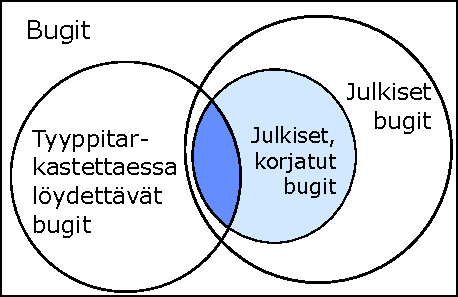
\includegraphics{images/to_type_or_not_to_type_venn.pdf}
\caption{To Type or Not to Type: Quantifying Detectable Bugs in JavaScript
         -tutkimuksen käsittelemät bugit \cite{ToTypeOrNotToType}.}
\label{fig:ToTypeOrNotToType}
\end{figure}

Kuva \ref{fig:ToTypeOrNotToType} luokittelee
tutkimuksessa \cite{ToTypeOrNotToType} kiinnostuksen kohteena
olleet ohjelmointivirheet. Tutkimuksessa käsiteltiin ainoastaan
julkisia, jo korjattuja bugeja. Suuri osa ohjelmointivirheistä jää
kuitenkin luultavasti tämän joukon ulkopuolelle, sillä ohjelmissa voi
olla bugeja joita kehittäjät eivät ole vielä havainneet ja joista
käyttäjät eivät ole ilmoittaneet. Esimerkiksi ohjelma \ref{lst:fridaybug}
saattaisi aiheuttaa vaikeasti havaittavan virheen joka jäisi helposti 
huomaamatta manuaalisesti tehtävässä testauksessa ja jopa yksikkötesteissä
\begin{lstlisting}[
  caption={Vaikeasti havaittavan virheen aiheuttava koodiesimerkki},
  label={lst:fridaybug}
]
if (viikonpaiva === "perjantai") {
  // Alennus perjantaisin 5 euroa
  ostoskori.lisääTuote({ nimi: "astiasto", Hinta: 10 });
} else {
  ostoskori.lisääTuote({ nimi: "astiasto", hinta: 15 });
}
\end{lstlisting}
Esimerkin \ref{lst:fridaybug} ei toimi oikein perjantaisin, sillä
\inlinecode{Ostos}-tyyppisen
objektin ominaisuus \inlinecode{hinta} on virheellisesti kirjoitettu isolla
alkukirjaimella. Koska bugi toistuu vain tietyissä olosuhteissa, se voi pysyä
havaitsemattomana pitkään. Staattinen analyysi etsii tyyppivirheitä
kaikista koodin haaroista ja tyyppiannotoituna kaikki kolme työkalua
pystyvätkin osoittamaan esimerkissä olevan virheen.

\section{Ohjelman optimointi käännösvaiheessa}
Aivan ensimmäiset tyyppijärjestelmät, kuten Fortranin (1957) staattinen tyypitys,
kehitettiin laskutoimitusten suoritusajan optimointia varten \cite{TypesAndProgrammingLanguages}.
Myös uudemmissa kielissä tyypeistä saatavilla olevaa tietoa
voidaan käyttää ajonaikaisen esimerkiksi turvallisuuden varmistavien
tarkistusten optimointiin.

Kun JavaScriptiä optimoidaan käännösvaiheessa, on kuitenkin usein hyödyllistä
kiinnittää enemmän huomiota tuotetun koodin kokoon kuin suoritusaikaiseen
tehokkuuteen. JavaScriptin yleisin käyttökohde ovat verkkosivut,
joissa selain lataa lähdekoodin sivulle saapuessa
internet-yhteyden yli juuri ennen ohjelman suorittamista. Ladattavan\newline
JavaScript-koodin määrä vaikuttaa siihen kauanko sivun lataus
kestää, joten koodin koon kasvattaminen minimaalisen suoritusajan
edun vuoksi ei usein ole kokonaisuudessaan hyödyllistä.
Closure–kääntäjä on kehitetty erityisesti
JavaScript-koodin koon optimointia ajatellen. Muuttujanimet voidaan helposti
uudelleennimetä ilmankin staattisen tyypityksen apua, mutta sen lisäksi
joukko muita koodia keventäviä optimointeja on käytettävissä kun kääntäjällä
on muuttujien tyypeistä saatava tieto käytettävissä. Closure–kääntäjä osaa
uudelleennimetä myös luokkamuuttujien nimiä lyhyemmiksi, poistaa
käyttämätöntä koodia, sekä korvata yksinkertaisia funktiokutsuja siirtämällä
funktion sisältämät ohjeet kutsuntapaikalle (engl. function inlining).

\begin{lstlisting}[
  caption={Esimerkki JavaScript-koodista jota Closure osaa optimoida},
  label={fig:optimoitava_javascript}
]
class HintaLaskuri {
	constructor() {
	  this.ostostenHintaYhteensa = 0
		this.arvonlisavero = 0.14
	}
	lisaaTuote(hinta) {
		this.ostostenHintaYhteensa += hinta
	}
	yhteensa() {
    return this.ostostenHintaYhteensa +
      this.ostostenHintaYhteensa * this.arvonlisavero
	}
}
const laskuri = new HintaLaskuri()
laskuri.lisaaTuote(5)
console.log(laskuri.yhteensa())
\end{lstlisting}
Esimerkissä \ref{fig:optimoitava_javascript} on yksinkertainen
JavaScript-tiedosto, jota Closure voi optimoida kooltaan pienemmäksi
ja ajonaikaiselta suorituskyvyltään nopeammaksi.
\begin{lstlisting}[
  caption={Closuren optimoima JavaScript-koodi},
  label={fig:optimoitu_javascript}
]
var $laskuri$$=new function(){this.$a$=0};
$laskuri$$.$a$+=5;
console.log($laskuri$$.$a$+.14*$laskuri$$.$a$);
\end{lstlisting}
Listauksessa \ref{fig:optimoitu_javascript} näkyy Closuren (versio 20190215.0.2)
tuottama koodi. Pitkä luokan \inlinecode{HintaLaskuri} jäsenmuuttuja
\inlinecode{ostostenHintaYhteensa} on uudelleennimetty lyhyeen muotoon
\inlinecode{\$a\$}. Closure näkee että luokan \inlinecode{HintaLaskuri}
metodeja kutsutaan \inlinecode{lisaaTuote} ja \inlinecode{yhteensa} kutsutaan
vain yhdessä kohdassa koodia, joten se on siirtänyt metodien ohjeet luokan
ulkopuolelle, alkuperäiselle kutsupaikalle, ja muuttanut parametriviittaukset
viittauksiksi alkuperäisen kutsun argumentteihin.\newline
\inlinecode{arvonlisavero}-luokkamuuttuja
on poistettu kokonaan ja korvattu käyttöpaikalla\newline
\inlinecode{.14} \textit{numeroliteraalilla},
mikä paitsi pienentää koodin kokoa myös saattaa parantaa suorituksenaikaista
tehokkuutta, sillä koodia suorittavan moottorin ei
tarvitse noutaa\newline
\inlinecode{arvonlisavero}-luokkamuuttujaa
luokan \textit{instanssista}. Käännöksen tulos on vaikeasti
luettavaa, mutta se onkin tarkoitettu JavaScript-moottorin suoritettavaksi
eikä ohjelmoijan luettavaksi. Ongelmatilanteissa, lopullista koodia
tutkittaessa, käännetty koodi voidaan palauttaa
alkuperäiseen muotoonsa ohjelmoijan luettavaksi käyttämällä \textit{lähdekarttoja}
(engl. source map) \cite{SourceMapMDN, SourceMapsDocsClosure},
jotka kuvaavat minimoidun lähdekoodin yhtymäkohtia alkuperäiseen.

\section{Tyyppimäärittelyt dokumentaationa}
Nykyaikasten editorien vakio-ominaisuuksiin kuuluu kirjoittamisen tukeminen
automaattisilla ehdotuksilla. Yksinkertaisimmillaan ehdotukset voivat
perustua avatuissa tiedostoissa käytettyihin sanoihin, joita editori ehdottaa
käytettäväksi uudelleen koodia kirjoitettaessa. Alkeellisetkin ehdotukset
voivat nopeuttaa kirjoittamista silloin kun ne sattuvat osumaan oikeaan,
mutta suurempi hyöty saadaan kun ehdotusten taustalla on syvempää koodin
analyysia. Kun editori tai ehdotukset tarjoava editorin lisätyökalu ymmärtää
koodissa olevia rakenteita ja niiden tyyppejä, ehdotukset ovat
täsmällisempiä ja perustuvat kontekstiin johon uutta koodia ollaan juuri
kirjoittamassa. Kuvassa \ref{fig:Suggestions} näkyy
\textit{VSCode}-editorin antamat ehdotukset eräille JavaScript-
ja TypeScript-tiedostoille.
TypeScriptiä kirjoittaessa editori ymmärtää että \inlinecode{tuote.}-ilmaisun
jälkeen ainoat järkevät ehdotukset ovat \inlinecode{Ostos}-tyyppisen muuttujan
ominaisuuksien nimiä, eli että ohjelmoija haluaa hyvin suurella todennäköisyydellä
kirjoittaa joko \inlinecode{tuote.hinta} tai \inlinecode{tuote.nimi}.
Ehdotuksen voi hyväksyä helposti enteriä painamalla, jolloin ehdotettua
koodinpätkää ei tarvitse kirjoittaa käsin.

Eksplisiittisesti kirjoitetut tyypit sekä editorin antama tieto muuttujien
tyypeistä voivat toimia myös aiemmin kirjoitetun koodin dokumentaationa ja
kuvauksena siitä, miten moduulia on tarkoitus käyttää.
Ehdotukset toimivat eräänlaisena dokumentaation lähteenä,
sillä ohjelmoija voi tutkia luokan tai
paketin tarjoamaa sisältöä ehdotettuja nimiä selaamalla. Automaattisia ehdotuksia
on mahdollista tarjota myös dynaamisesti tyyppitarkastetuille kielille, mutta
koodipohjan kasvaessa ja muuttuessa monimutkaisemmaksi ehdotusten tarkkuus
on vaikea pitää samalla tasolla kuin staattisesti tyypitetyissä kielissä.
Huonoimmillaan ehdotetut muuttuja- ja metodinimet valitaan yksinkertaisesti
listaamalla avoimista tiedostoista löytyviä nimiä, välittämättä sen
enempää siitä onko nämä metodit määritetty juuri kyseiselle tyypille.
Edistyneemmät ehdotusmoottorit, kuten Visual Studiossa käytetty IntelliSense,
suorittavat osaa JavaScript-koodista taustalla ja analysoivat siten muuttujien
tyyppejä ajonaikana \cite{PreviewingSalsa, JavaScriptIntellisense}.
Tämä tekniikka yhdistettynä tavanomaisempaan tyyppien
käännösaikaiseen päättelyyn voi riittää tarjoamaan melko kattavan kuvauksen
jonkin muuttujan tyypistä, mutta jää silti jälkeen siitä tarkkuudesta jonka
IntelliSense osaa antaa staattisesti tyypitetylle koodille.
\begin{figure}
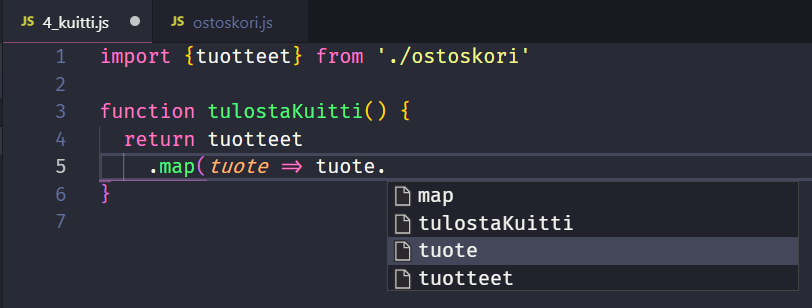
\includegraphics[width=0.8\textwidth]{images/intellisense_javascript}
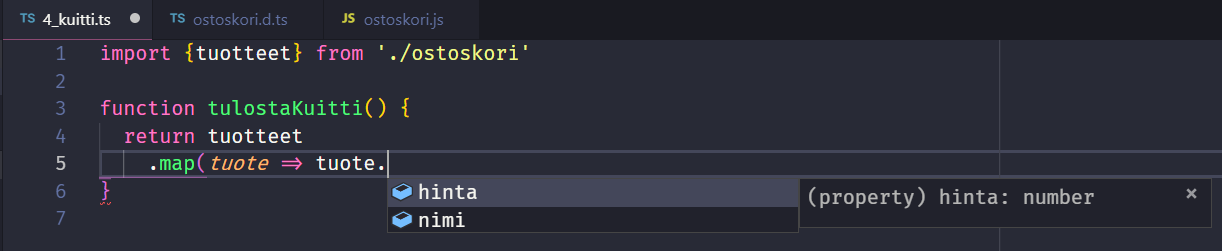
\includegraphics[width=\textwidth]{images/intellisense_typescript}
\noindent
\caption{
  VSCode-editorin tarjoamat ehdotukset JavaScriptille (yllä) ja TypeScriptille (alla).
  JavaScriptille annetuissa ehdotuksissa on turhia, tiedostossa käytettyihin
  sanoihin perustuvia ehdotuksia.}
\label{fig:Suggestions}
\end{figure}

Automaattisten ehdotusten vaikutuksesta ohjelmointityön tehokkuuteen ei
kuitenkaan ole yleisesti hyväksyttyä, tutkittua varmuutta. Vaikka metodien
nimet olisivatkin ohjelmoijan nähtävillä editorissa, ne eivät välttämättä
sellaisenaan tarjoa tarpeeksi hyötyä dokumentaationa jotta työtehokkuus
kasvaisi merkittävästi. Vuonna 2015 toteutettu tutkimus
``An Empirical Investigation of the Effects of Type Systems and Code Completion
on API Usability using TypeScript and JavaScript in MS Visual Studio''
testasi staattisen tyypityksen ja automaattisten ehdotusten tehokkuutta
antamalla osallistujille toteutettavaksi ohjelmointitehtävän JavaScriptillä
ja TypeScriptillä, automaattisten ehdotusten kanssa ja niitä ilman
\cite{EmpiricalInvestigationOfCodeCompletion}. Tutkimuksen mukaan
automaattiset ehdotukset eivät toisi tilastollisesti merkittävää parannusta
ohjelmointitehtävän ratkomisnopeuteen. Samassa tutkimuksessa kuitenkin nähtiin
että TypeScriptiä käyttäneet koehenkilöt suoriutuivat tehtävästä nopeammin,
automaattisilla ehdotuksilla tai ilman. Voi olla, että automaattisia ehdotuksia
tehokkaampi työkalu on itse kääntäjä, joka paljastaa virheet koodissa ennen
kuin ohjelmoijan tarvitsee kokeilla koodin toimivuutta käytännössä.
